\documentclass[10pt]{article}
\usepackage[a4paper, total={7in,10in}]{geometry}
\usepackage{hyperref}
\usepackage{siunitx}
\usepackage{graphicx}
\usepackage{caption}
\usepackage[backend=biber]{biblatex}
\addbibresource{report.bib}

%opening
\title{EP2420 Project 1 - Advanced Project}
\author{André Silva}
\begin{document}

\maketitle

\section*{Project Overview}
\label{sec:1}

In this project, we train machine learning models, namely \textit{Linear Regression}, \textit{Random Forest Regression}, \textit{Neural Network Regression}, and \textit{Random Forest Classification}, that map infrastructure measurements of a networked service to service-level metrics.

We conduct several experiments to measure the performance of these models conditional to the utilization of pre-processing techniques such as \textit{L2 Normalization}, \textit{Restriction to Interval}, \textit{Standardization}, \textit{Outlier Removal}, and \textit{Discretization}.

With the results from the different experiments, we find that pre-processing and data manipulation enables models to perform more accurately when predicting unseen data.

\section*{Background}
\label{sec:2}

We will be analyzing the data set \textit{VoD flash-crowd}, using the low-level infrastructure measurements to predict the video frame rate observed by clients.

The dataset was recorded on a test-bed running a \textit{Video-on-Demand (VoD)} service, with a load generator following a \textit{flash-crowd} pattern where the load level peaks at certain flash events.

More information on the infrastructure and specificities of the dataset can be found in ~\cite{9012741}.

\section*{Task I}
\label{sec:3}

In this task we aim at providing an overview of the dataset, describing some relevant statistics on a sample of features and the target metric, as well as explain what said features mean.

The dataset \textit{VoD flash-crowd} provides us with $36633$ samples of $1670$ features, and $9$ different types of targets.

In Table \ref{table:1}, the statistics for the chosen features, as well as the target \textit{DispFrames}, which represents the video frame rate, are displayed.

\begin{table}[h!]
    \centering
    \begin{tabular}{ | c | c | c | c | c | c | c | }
        \hline
        Feature name & Mean & Std Dev & Maximum & Minimum & 25th percentile & 90th percentile \\ 
        \hline
        \textit{3\_cpu16\_.sys} & \num{3.55e+00} & \num{1.95e+00} & \num{1.50e+01} & \num{0.00e+00} & \num{0.00e+00} & \num{0.00e+00} \\
        \hline
        \textit{23\_RxPacktes} & \num{3.15e+02} & \num{4.12e+02} & \num{2.37e+03} & \num{0.00e+00} & \num{3.70e+01} & \num{4.70e+01} \\
        \hline
        \textit{3\_frmpg.s} & \num{-1.15e+01} & \num{2.07e+04} & \num{1.08e+05} & \num{-7.49e+04} & \num{-5.31e+04} & \num{-4.55e+04} \\
        \hline
        \textit{0\_cpu18\_.idle} & \num{9.97e+01} & \num{5.98e-01} & \num{1.00e+02} & \num{9.50e+01} & \num{9.70e+01} & \num{9.80e+01} \\
        \hline
        \textit{2\_cpu17\_.usr} & \num{6.03e+01} & \num{1.82e+01} & \num{9.20e+01} & \num{0.00e+00} & \num{8.00e+00} & \num{1.34e+01} \\
        \hline
        \textit{4\_cpu15\_.iowait} & \num{4.65e-03} & \num{7.21e-02} & \num{3.03e+00} & \num{0.00e+00} & \num{0.00e+00} & \num{0.00e+00} \\
        \hline
        \textit{4\_cpu5\_.sys} & \num{2.90e+01} & \num{1.08e+01} & \num{7.40e+01} & \num{0.00e+00} & \num{6.06e+00} & \num{9.18e+00} \\
        \hline
        \textit{3\_cswch.s} & \num{7.30e+04} & \num{1.79e+04} & \num{1.07e+05} & \num{7.82e+03} & \num{2.19e+04} & \num{2.65e+04} \\
        \hline
        \textit{38\_TxBytes} & \num{2.79e+06} & \num{3.18e+06} & \num{1.96e+07} & \num{0.00e+00} & \num{3.47e+05} & \num{4.63e+05} \\
        \hline
        \textit{2\_dev8.0\_avgrq.sz} & \num{2.21e+01} & \num{5.78e+01} & \num{1.02e+03} & \num{0.00e+00} & \num{0.00e+00} & \num{0.00e+00} \\
        \hline
        \textit{DispFrames} & \num{2.20e+01} & \num{4.32e+00} & \num{2.50e+01} & \num{0.00e+00} & \num{3.00e+00} & \num{8.00e+00} \\
        \hline
    \end{tabular}
    \caption{Statistics for chosen features and target}
    \label{table:1}
\end{table}

The following list gives a short description of these features. This information was retrieved from linux manual pages for the command \texttt{sar}~\cite{sar}.

\begin{itemize}
    \item \textit{3\_cpu16.sys} - Percentage of CPU utilization that occurred while executing at the system level (kernel).
    \item \textit{23\_RxPackets} - Total number of packets received per second.
    \item \textit{3\_frmpg.s} - Number of memory pages freed by the system per second.
    \item \textit{0\_cpu18\_.idle} - Percentage of time that the CPU or CPUs were idle and the system did not have an outstanding disk I/O request.
    \item \textit{2\_cpu17\_.usr} - Percentage of CPU utilization that occurred while executing at the user level (application).
    \item \textit{4\_cpu15\_.iowait} - Percentage of time that the CPU was idle during which the system had an outstanding disk I/O request.
    \item \textit{4\_cpu5\_.sys} - Percentage of CPU utilization that occurred while executing at the system level (kernel).
    \item \textit{3\_cswch.s} - Total number of context switches per second.
    \item \textit{38\_TxBytes} - Total number of bytes transmitted per second.
    \item \textit{2\_dev8.0\_avgrq.sz} - The average size (in sectors) of the requests that were issued to the device.
\end{itemize}

\section*{Task II}
\label{sec:4}

\subsection*{2.1}
\label{sec:5}

Table \ref{table:2} provides the calculated \textit{Normalized Mean Absolute Error} (\textsc{NMAE}) for each of the regressors.
The parameters utilized for the random forest regression and the neural network regression are the default parameters of, respectively, \texttt{RandomForestRegressor}~\cite{RFR} and \texttt{MLPRegressor}~\cite{MLPR}, unless specified in the table.
\begin{table}[h!]
    \centering
    \begin{tabular}{ | c | c | c | }
        \hline
        Regressor & \textsc{NMAE} & Training time (in seconds) \\ 
        \hline
        \texttt{LinearRegression} & \num{0.318} & \num{5.09}\\ 
        \hline
        \texttt{RandomForestRegressor(n\_estimators=10)} & \num{0.087} & \num{1.24e+02} \\ 
        \hline
        \texttt{MLPRegressor(max\_iter=1000, act='logistic', hidden\_layers=(10,10))} & \num{0.144} & \num{5.50e+01}\\ 
        \hline
    \end{tabular}
    \caption{\textit{Normalized Mean Absolute Error} for each regressor tested}
    \label{table:2}
\end{table}

\begin{figure}[h!]
    \centering
    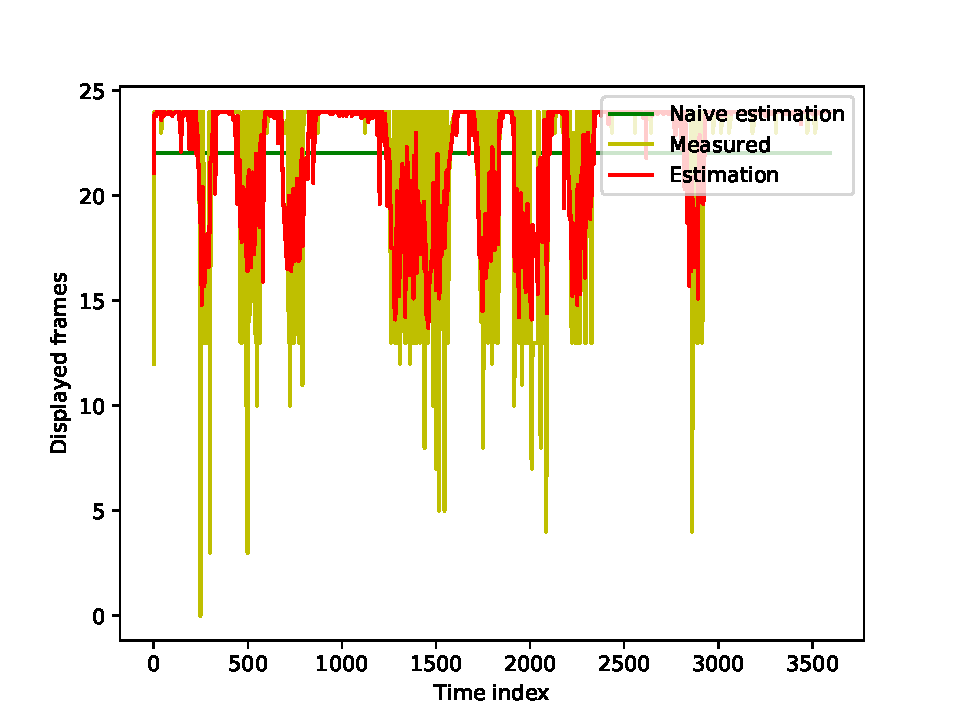
\includegraphics[width=0.72\textwidth,height=\textheight,keepaspectratio]{../result/project1/rfr.pdf}
    \caption{Time series plot for \textit{VoD flashcrowd} using \textit{RandomForestRegressor}}
    \label{fig:1}
\end{figure}

\begin{figure}
    \centering
    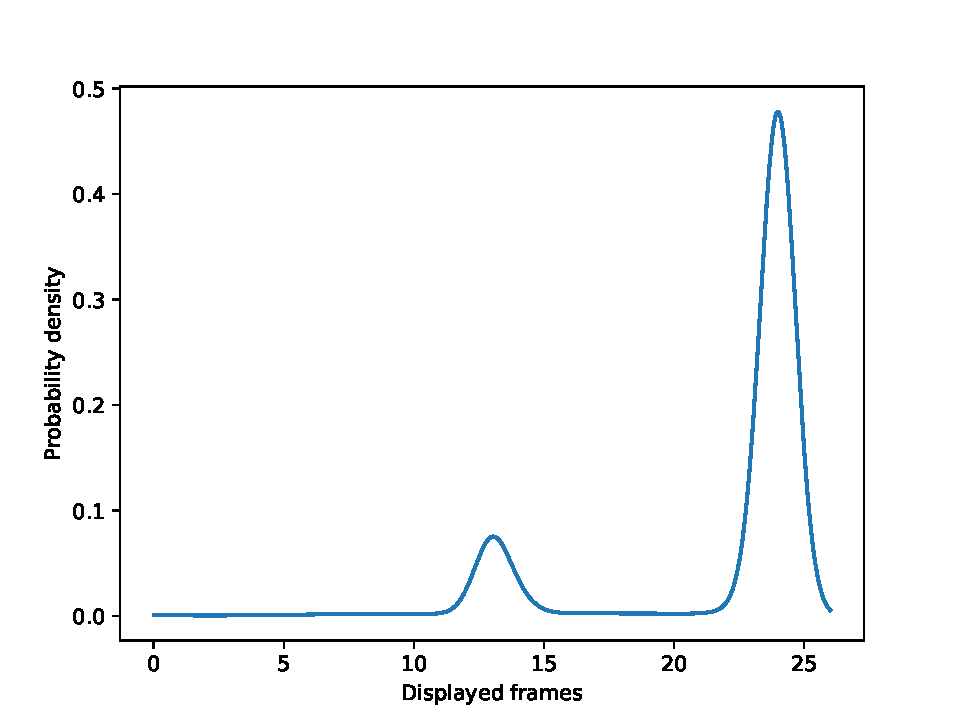
\includegraphics[width=\textwidth,height=0.25\textheight,keepaspectratio]{../result/project1/frames_density.pdf}
    \caption{Density plot of the target values in the test set}
    \label{fig:2}
\end{figure}

\begin{figure}
    \centering
    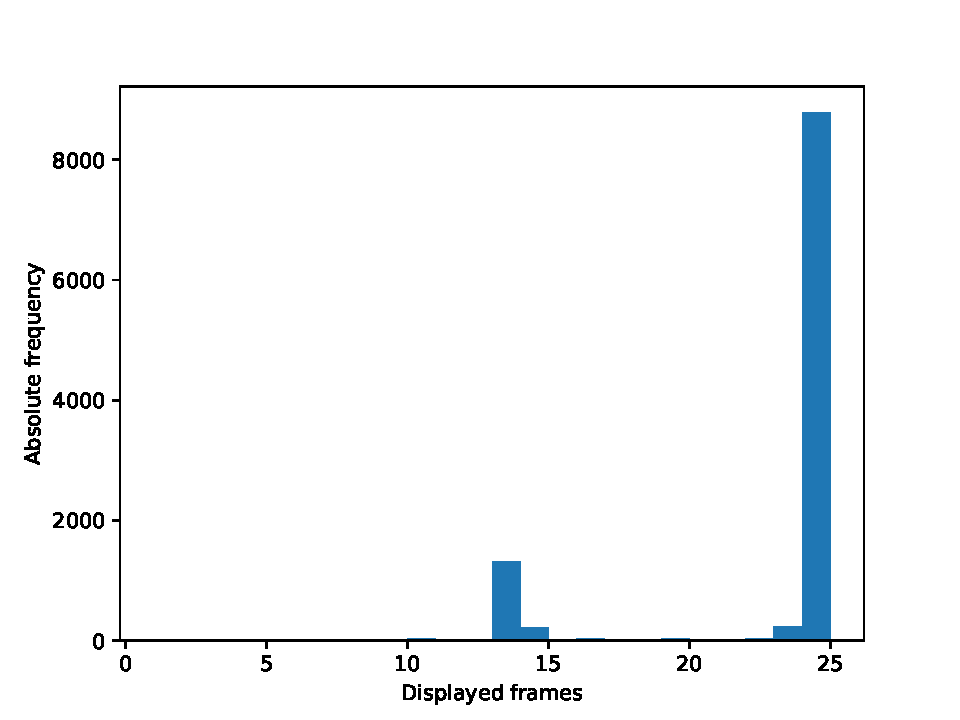
\includegraphics[width=\textwidth,height=0.25\textheight,keepaspectratio]{../result/project1/frames_hist.pdf}
    \caption{Histogram of the target values in the test set}
    \label{fig:3}
\end{figure}

\begin{figure}
    \centering
    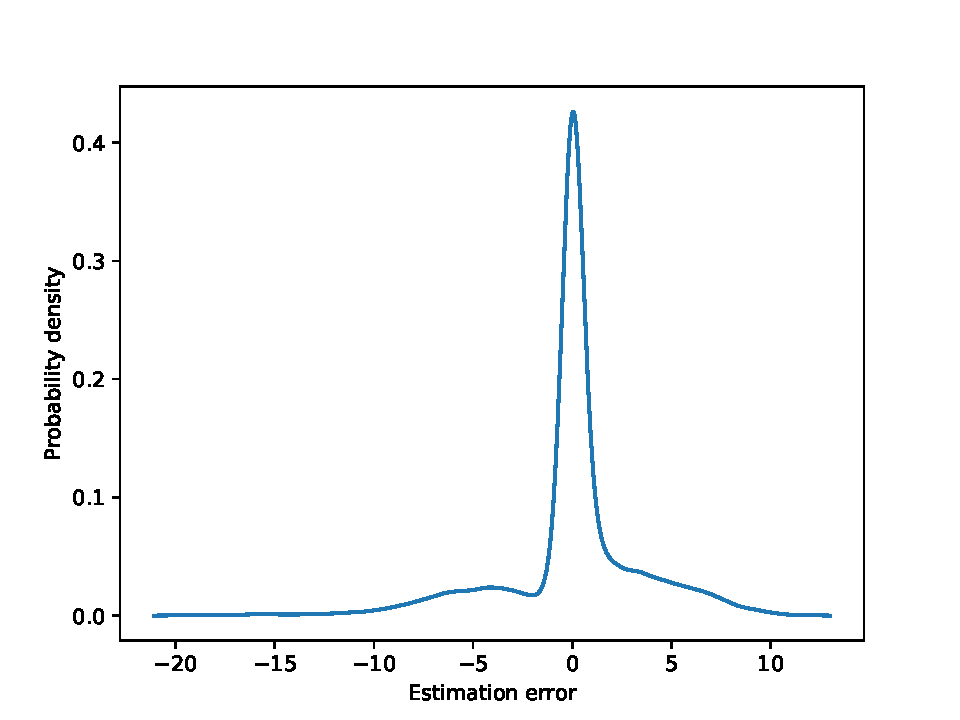
\includegraphics[width=\textwidth,height=0.25\textheight,keepaspectratio]{../result/project1/error_density.pdf}
    \caption{Density plot of the estimation errors $y_i - \hat{y}_i$ in the test set using \textit{RandomForestRegressor}}
    \label{fig:4}
\end{figure}

\clearpage

By looking at the results in Table ~\ref{table:2}, we can see that, of the three regression techniques utilized, \textit{Linear Regression} provided the worst accuracy, while being the least expensive in terms of training time. \textit{Neural Network Regression} was less expensive than \textit{Random Forest Regression}, which was the most expensive but also the one which provided the best results.

The bad results of \textit{Linear Regression} can be partially explained by the impact outliers have on this type of models, as we used a regular least squares regression and the lack of pre-processing. The same can be said about \textit{Neural Network Regression}, where we also note that the hyper-parameters utilized play a significant role and could, if further investigated, allow this model to outperform \textit{RandomForestRegression}. Random Forests are, on the other hand, known to perform out-of-the-box, meaning hyper-parameters and pre-processing of data usually don't result in major improvements when compared to the default and unprocessed data models.

In Figure \ref{fig:1} we can see the time series plot of the first 3600 seconds. In red we plot the predicted predicted target values, in yellow the measured target values and in green the mean value.
We can see that the model can accurately predict when the target value drops from $24$, but fails to predict most values lower than $15$. 
By looking at Figures \ref{fig:2} and \ref{fig:3}, we notice that observed target values fluctuate between 24 and 13, which could indicate that the system has a control system that triggers a lower frame rate when load reaches a certain level. This is also what we observe in the measured curve in Figure \ref{fig:1}.

\subsection*{2.2}
\label{sec:6}

\begin{figure}[h!]
    \centering
    \captionsetup{justification=centering}
    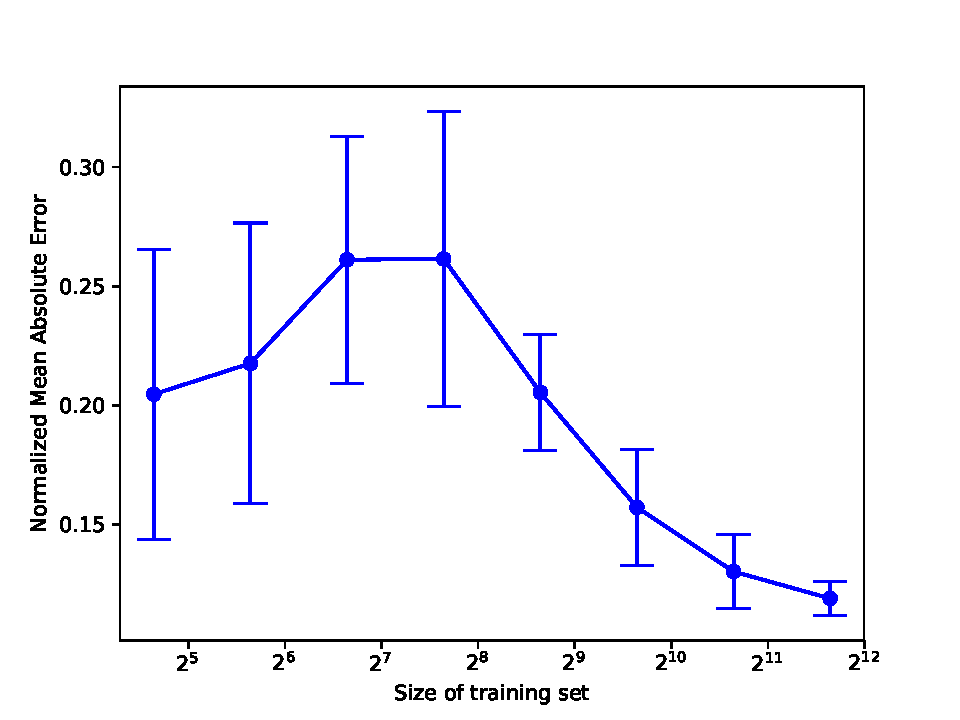
\includegraphics[width=0.72\textwidth,height=\textheight,keepaspectratio]{../result/project1/training_set_size_errors.pdf}
    \caption{Measured \textit{Normalized Mean Absolute Error} for a given training set size using \textit{Lasso Regression}~\cite{Lasso}. Error bars represent $2\sigma$ over 50 measurements. Data points represent means.}
    \label{fig:5}
\end{figure}

Intuition tells us that the more information we have access to, the better conclusion we can extract from them.

In Figure \ref{fig:5}, we can find the results of our experiment to prove this assumption. The blue dots represent means over 50 measurements for each training set size, while errors bars represent $2\sigma$. By looking at it, we notice that the curve begins by unexpectedly increasing, followed by an expected decrease. 

We can also notice that the variance of the measurements starts off very high, and shows a decreasing tendency as we increase the size of the training set. This partly explains why the curve doesn't follow our initial expectations. 

Another reason that can explain this is the fact that outliers in small training sets have a higher influence than in large training sets, and the probability of including outliers in randomly picked training sets decreases as we decrease its size.

Overall, we can conclude that the larger a training set is the better a model can predict the system, as the training set becomes more general and so more information can be inferred from it.

\section*{Task III}
\label{sec:7}

\begin{figure}[h!]
    \centering
    \captionsetup{justification=centering}
    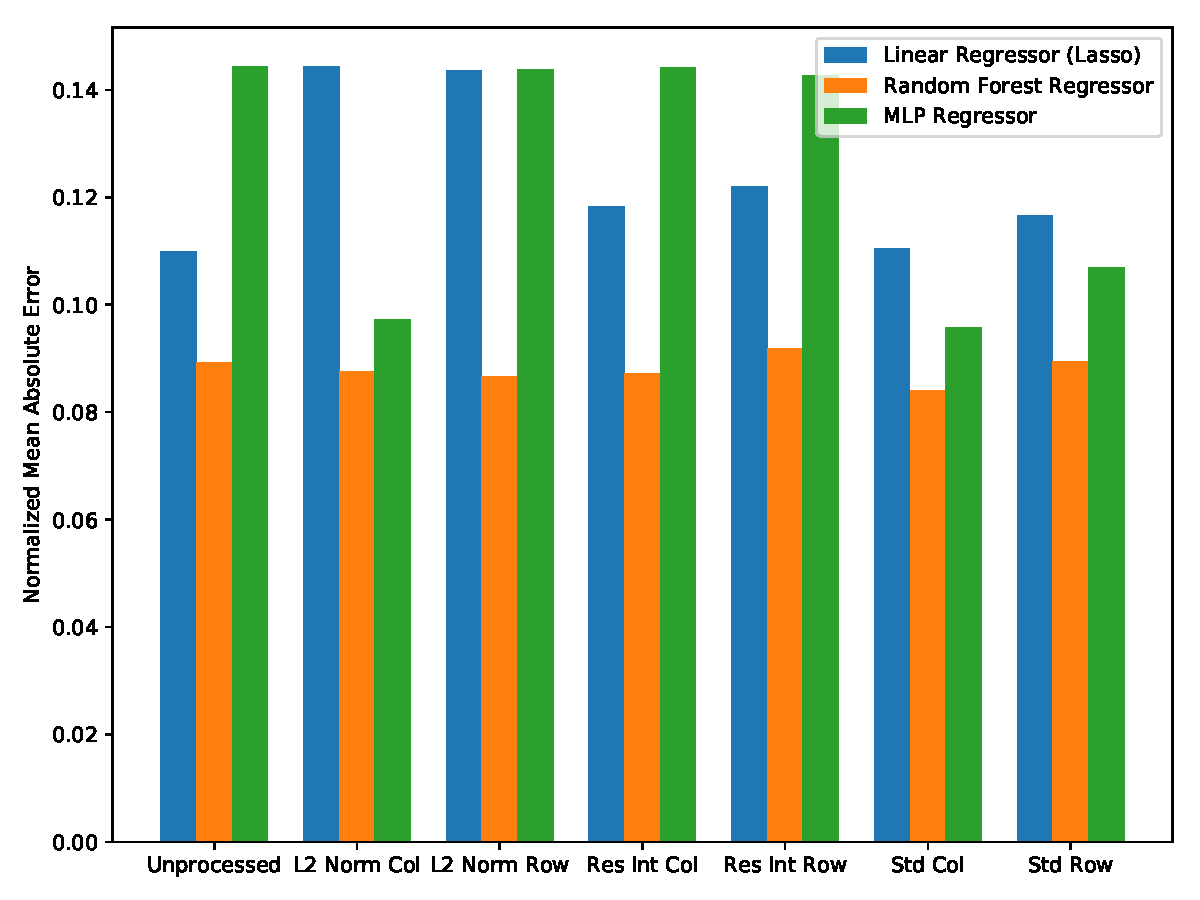
\includegraphics[width=0.72\textwidth,height=\textheight,keepaspectratio]{../result/project1/pre_processing_accuracies.pdf}
    \caption{Measured \textit{Normalized Mean Absolute Error} for a given pre-processed dataset.}
    \label{fig:6}
\end{figure}

In Figure \ref{fig:6}, we present the results of our experiment with the objective of evaluating the impact of pre-processing techniques on the considered machine learning models' accuracy.

We can see that pre-processing the data impacts some models more than others.
In the case of \textit{Random Forest Regression}~\cite{RFR}, the gains or losses of accuracy are marginal for all pre-processing methods. This happens by definition, since tree partition algorithms are not affected by the scaling or centralization of datapoints.

\textit{MLP Regressor}~\cite{MLPR} seems to be the model which suffers the biggest impact from data pre-processing, showing either no difference or a considerable gain.

\textit{Lasso}~\cite{Lasso} consistently shows worse performance on pre-processed data when compared to the original one.

By analyzing Figure \ref{fig:6} again, we can see that standardizing along each column is the method that results in the best results for all 3 regression techniques.

\pagebreak

\begin{figure}[h!]
    \centering
    \captionsetup{justification=centering}
    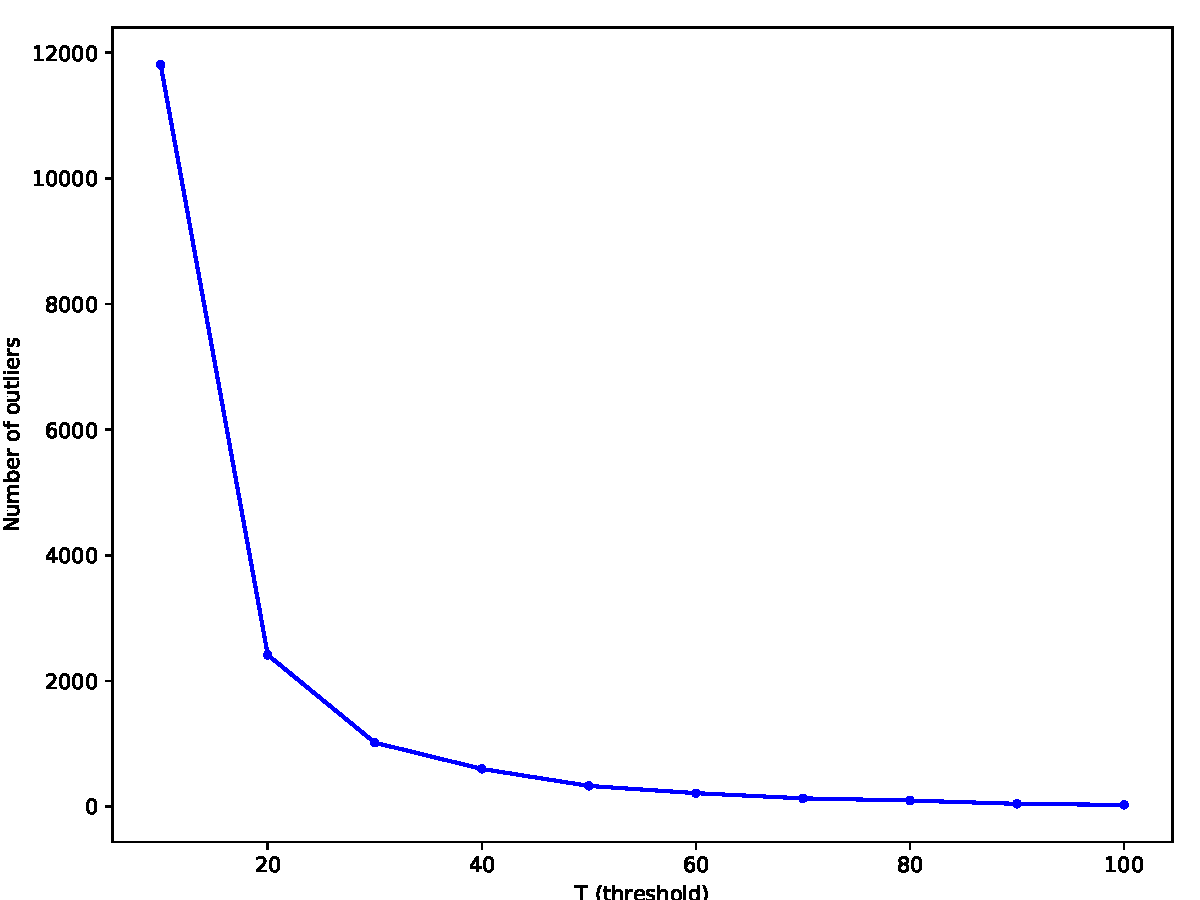
\includegraphics[width=0.65\textwidth,height=\textheight,keepaspectratio]{../result/project1/number_outliers.pdf}
    \caption{Number of outlier points for a given threshold on the standardized design matrix along each column.}
    \label{fig:7}
\end{figure}

\begin{figure}[h!]
    \centering
    \captionsetup{justification=centering}
    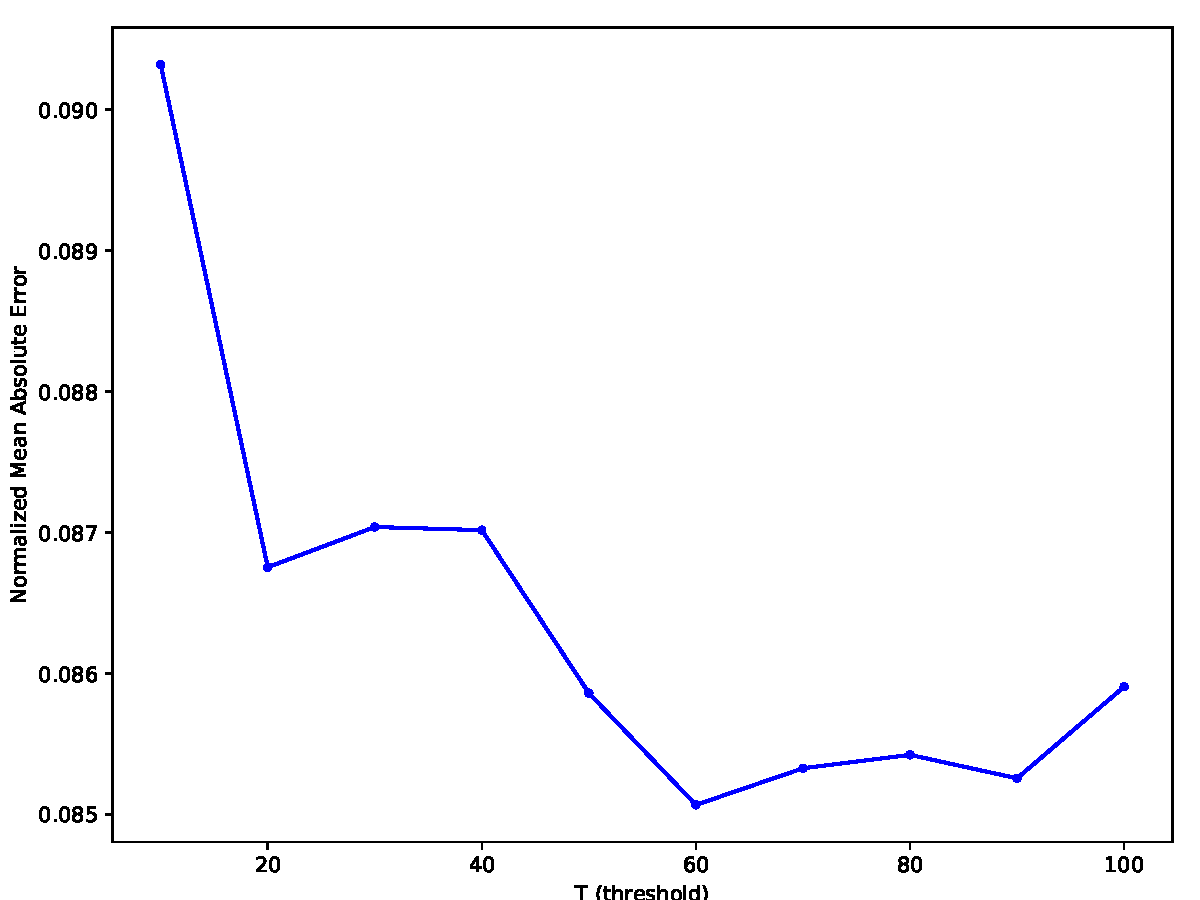
\includegraphics[width=0.65\textwidth,height=\textheight,keepaspectratio]{../result/project1/nmae_outliers.pdf}
    \caption{\textit{Normalized Mean Absolute Error} for a given threshold T (outlier removal) using \textit{Random Forest Regression}~\cite{RFR}.}
    \label{fig:8}
\end{figure}

In Figures \ref{fig:7} and \ref{fig:8} we plot the results of our experiment with the purpose of measuring the impact of outlier removal on the accuracy of our model. Figure \ref{fig:7} plots the number of outliers removed for a given threshold (deviation from mean). Figure \ref{fig:8} plots the \textsc{NMAE} for a given threshold using \textit{Random Forest Regression}.

Figure \ref{fig:7} shows, as expected, a function that decreases while T increases, eventually converging to 0. This happens because we have standardized the data along each column, making each feature space look like a Gaussian distribution with 0 mean and unit variance.

As we filter rows based on absolute values, we will find less and less examples of outliers as T increases, by the definition of a Gaussian distribution.

Figure \ref{fig:8} shows us that the \textit{NMAE} starts off by decreasing, as we increase the threshold for outlier removal, suggesting low threshold values may lead to the removal of important parts of the dataset. As we incorporate more datapoints in our dataset, we can better predict outcomes. This goes in hand with the results of Task 2.1.

As we reach a very high treshold we notice a slight increase, which might represent the impact more extreme outliers have on the outcome of the tested model, \textit{Random Forest Regression}~\cite{RFR}. This approximation to a parabola was the expected result for this experiment.

\section*{Task IV}
\label{sec:8}

In this task we apply discretization into bins to the target value, video frame rate, with the intuit of predicting the distribution of said metric and later, in Task V, its percentiles.

Since we are analysing \textit{VoD flash-crowd}, we are going to convert our target values into an histogram of 31 labels, with midpoints 0, 1, 2, ..., 30.

\begin{figure}[h!]
    \centering
    \captionsetup{justification=centering}
    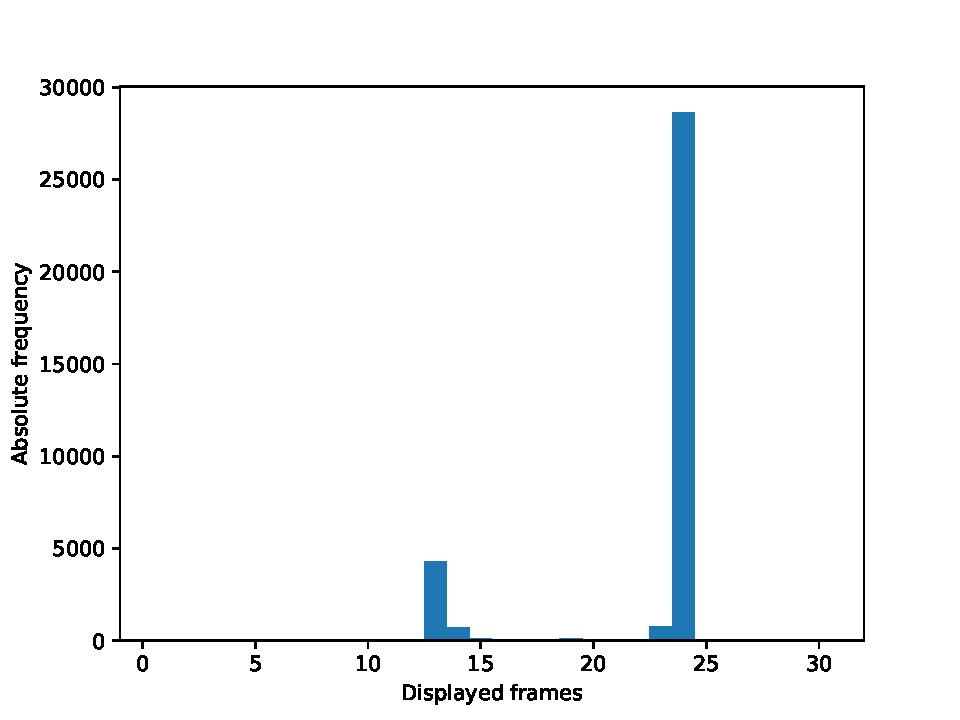
\includegraphics[width=0.72\textwidth,height=\textheight,keepaspectratio]{../result/project1/discretized_frames_hist.pdf}
    \caption{Histogram of the video frame rate on the interval $y\in[-0.5,30.5]$, with a bin size of 1}
    \label{fig:9}
\end{figure}

We then take each bin of the histogram as a class and fit a \textit{RandomForestClassifier}~\cite{RFC} to the data, which has been target of standardization by column and outlier removal. The hyper-parameters used are the default ones, apart from the number of estimators, which was $10$. We train and test the model on a 70-30 split, as was the case for previous tasks.

The calculated \textsc{NMAE} for this model was approximatly $7.3\%$. In Task II, we had been able to train a model which got $8.7\%$ \textsc{NMAE}, which was then marginally improved in Task III. 

We can conclude by these results that the discretization of our target values allows us to better predict them. The loss of information as a result of this process is negligible, given the nature of the target values.

\pagebreak

\begin{figure}[h!]
    \centering
    \captionsetup{justification=centering}
    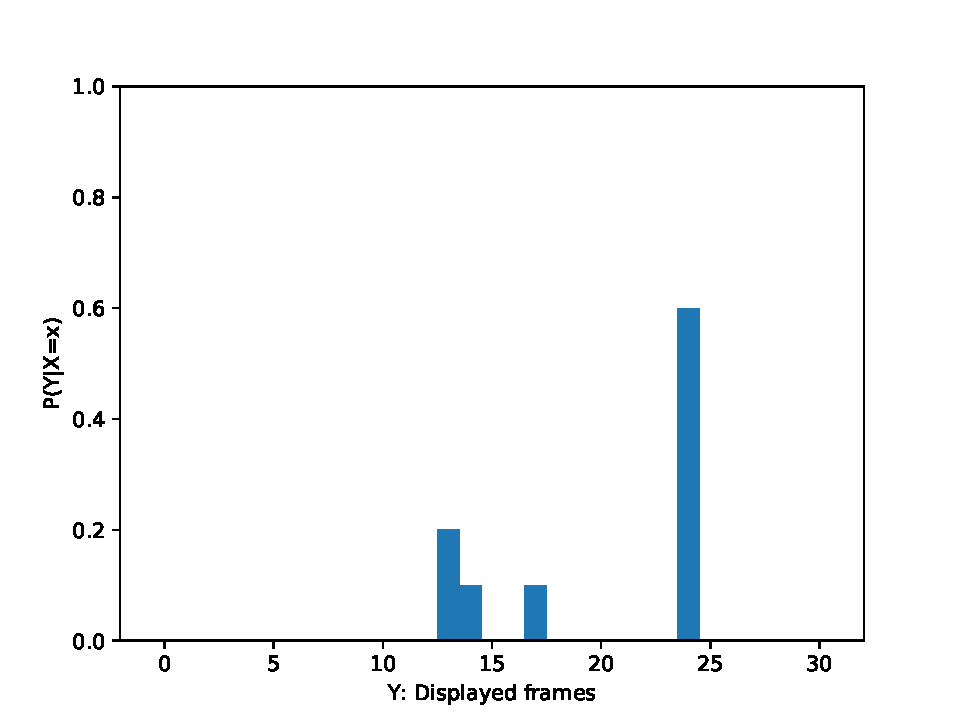
\includegraphics[width=0.72\textwidth,height=\textheight,keepaspectratio]{../result/project1/P(Y|X=x)_2643.pdf}
    \caption{Predicted histogram for a randomly selected sample of the test set. The measured target value was $24.0$}
    \label{fig:10}
\end{figure}

\begin{figure}[h!]
    \centering
    \captionsetup{justification=centering}
    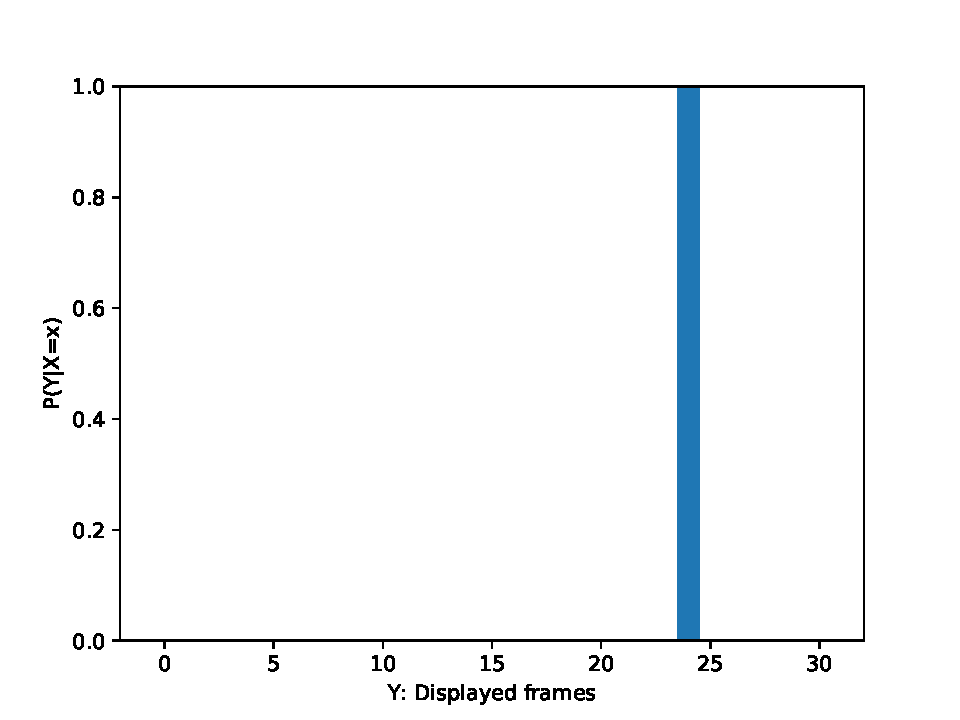
\includegraphics[width=0.72\textwidth,height=\textheight,keepaspectratio]{../result/project1/P(Y|X=x)_7272.pdf}
    \caption{Predicted histogram for a randomly selected sample of the test set. The measured target value was $24.0$}
    \label{fig:11}
\end{figure}

In Figures \ref{fig:10} and \ref{fig:11}, we can see the predicted histograms for two randomly selected samples of the test set, both with a measured value of $24.0$.

In the first case, $P(Y|X)$ is distributed between four classes, 13, 14, 17 and 24, whereas in the second case it is concentrated entirely on class 24. 
We can extract from this that, when the system is in a state equivalent to the first sample, it is, predictably, more unstable relative to the second, and that we can expect some disturbances in the video frame rate registered by the client.

\section*{Task V}

In this task, we take the histogram prediction build in Task IV and use it to predict percentiles of the target metric.

To predict the percentile values, we need to convert our bins into cumulative bins, so that every bin now represents $P(Y \le y|X = x)$. We can then, given a certain percentile $P_i$, say the predicted percentile is the value corresponding to the first cumulative bin with a value greater or equal to $P_i$.

\begin{figure}[h!]
    \centering
    \captionsetup{justification=centering}
    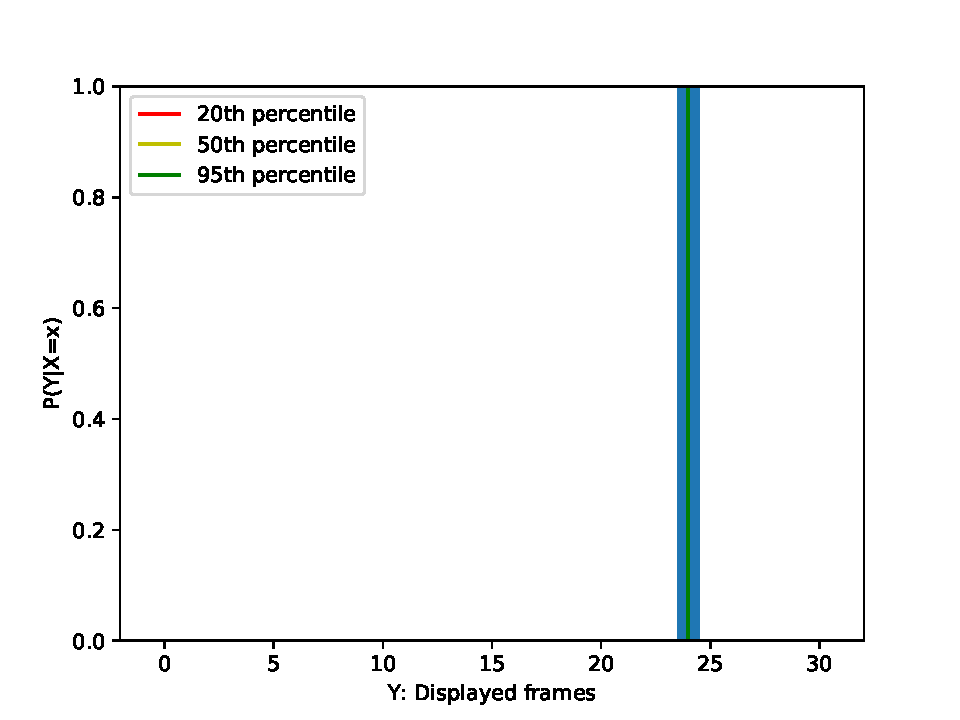
\includegraphics[width=0.72\textwidth,height=\textheight,keepaspectratio]{../result/project1/P(Y|X=x)_1192_percentiles.pdf}
    \caption{Predicted histogram with percentiles for a randomly selected sample of the test set. The measured target value was $24.0$}
    \label{fig:12}
\end{figure}

\begin{figure}[h!]
    \centering
    \captionsetup{justification=centering}
    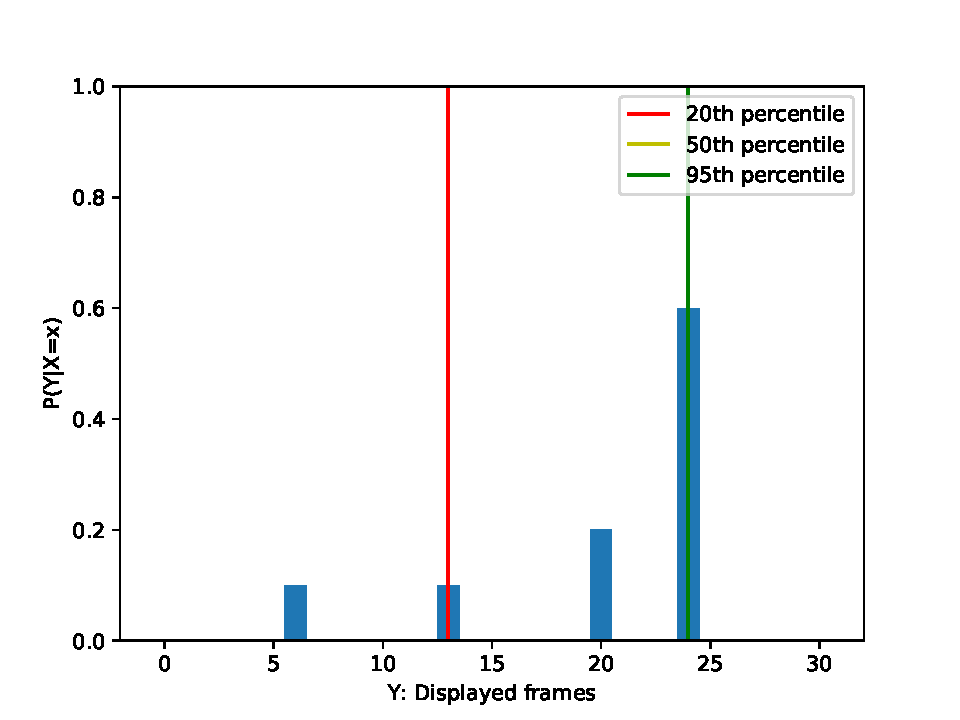
\includegraphics[width=0.72\textwidth,height=\textheight,keepaspectratio]{../result/project1/P(Y|X=x)_8597_percentiles.pdf}
    \caption{Predicted histogram with percentiles for a randomly selected sample of the test set. The measured target value was $23.0$}
    \label{fig:13}
\end{figure}

Figures \ref{fig:12} and \ref{fig:13} show the predicted histograms for two randomly selected samples of the test set. In red we can see the predicted 20th percentile, yellow the 50th and green the 95th.

Since the histogram is distributed along a small number of bins, we can see that some percentiles fall in the same bin. Figure \ref{fig:12} represents an extreme case, where the probability mass function is concentrated in a single bin.

\begin{figure}[h!]
    \centering
    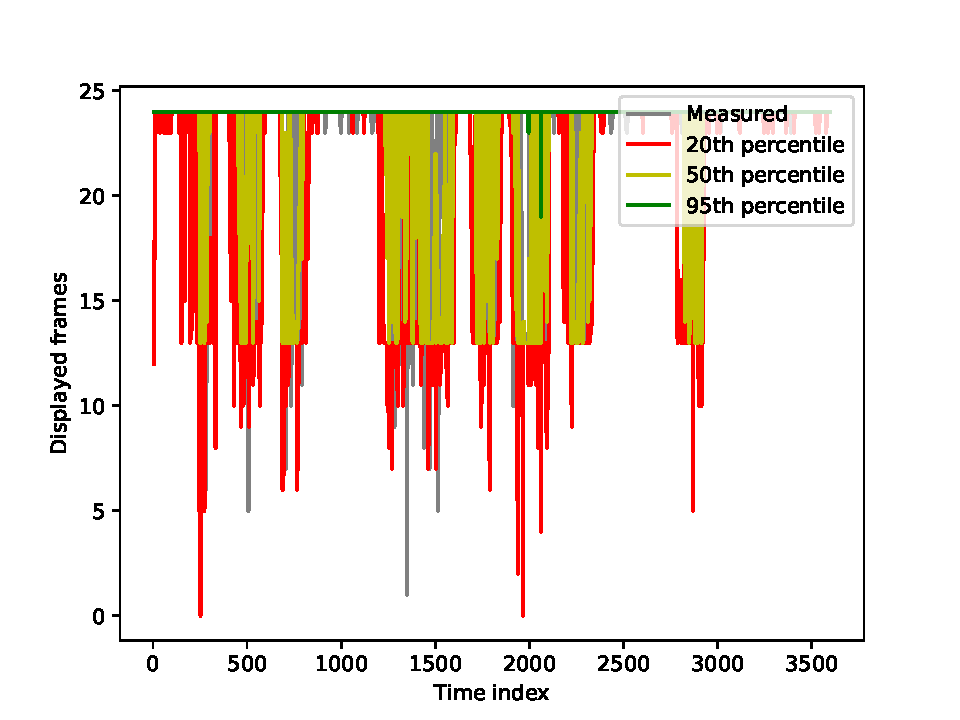
\includegraphics[width=0.72\textwidth,height=\textheight,keepaspectratio]{../result/project1/percentiles_timeplot.pdf}
    \caption{Time series plot for \textit{VoD flashcrowd} including predicted percentiles.}
    \label{fig:14}
\end{figure}

Figure \ref{fig:14} shows us the time series plot of our dataset for the first 3600 seconds. In gray we can see the measured values, in red the 20th percentile, yellow the 50th and green the 95th.

The percentile curves follow our expectations. The 20th percentile curve reaches the lowest levels of the measured metric, while the 95th percentile almost never drops from the value $24$. The 50th percentile curve fluctuates mostly between $13$, $14$, and $24$, which are the most common occurrences of the target metric, as shown in Figure \ref{fig:9}.

\begin{table}[h!]
    \centering
    \begin{tabular}{ | c | c | }
        \hline
        Percentile & Estimation of percentile \\ 
        \hline
        20th percentile & \num{0.703} \\ 
        \hline
        50th percentile & \num{0.895}\\ 
        \hline
        90th percentile & \num{0.999}\\ 
        \hline
    \end{tabular}
    \caption{Percentiles and the correspondent estimations.}
    \label{table:3}
\end{table}

In Table \ref{table:3}, we can see the estimations for each percentile using the provided formula.

We can see that none of the estimations are very accurate, since we were expecting values close to, respectively, $0.2$, $0.5$ and $0.9$.

Taking into account the conclusions regarding Figures \ref{fig:12} and \ref{fig:13}, where we saw that percentiles often fell in the same bins (as can also be confirmed by Figure \ref{fig:14}), we can conclude that our discretization process and the model's histogram prediction limits our estimations, as a sample that falls into a certain percentile can also, very likely, fall into a different percentile at the same time.

\section*{Discussion}

In Task I, we investigated relevant statistics of our dataset, a sample of features and the target value. We also discovered what the sampled features mean in the context of the networked system.

In Task II, we aimed at building three different models for predicting the target value and found that our \textit{RandomForestRegressor} behaved the best. We also studied the impact of training set size on the accuracy of a Lasso Regressor, reaching the conclusion that the more data we have for training the better we can predict the behavior of the system.

In Task III, we studied the impact of data pre-processing and outler removal on the performance of our models. We found that standardizing along each column was the method that provided the best results, improving accuracy on Linear Regression and Neural Network Regression, while Random Forest Regression was not impacted by any pre-processing technique. We also found that outlier removal enabled our \textit{RandomForestRegressor} to better predict, as long as we choose a reasonable threshold.

In Task IV, we predicted the distribution of our target metric using histrograms. We accomplished this by, first, discretizing our target metric into bins and then building a \textit{RandomForestClassifier}. The accuracy of this model represented an improvement when compared to the models of previous tasks. We then selected two samples of the test set to demonstrate the predicted histogram.

In Task V, we predicted percentiles of our target metric using the model built in the previous task. We concluded that, due to the discretization and nature of the dataset, predicted percentiles often fall in the same bin (or class). We confirmed these results when our estimation of the percentiles produced inaccurate results.

The main difficulties encountered during this project were related to the size of the dataset, which resulted in significant computational overhead during some experiments.

Further work can include the incorporation of more machine learning techniques, such as dimensionality reduction and more deep model selection, with the objective of improving accuracies and obtain a better understanding of the system

\printbibliography

\end{document}
